\documentclass[10pt,
%superscriptaddress,
%groupedaddress,
%unsortedaddress,
%runinaddress,
%frontmatterverbose, 
%preprint,
%preprintnumbers,
%nofootinbib,
%nobibnotes,
%bibnotes,
 amsmath,amssymb,
 aps,prb, twocolumn
]{revtex4-2}

% Graphics and math
\usepackage{graphicx}
\usepackage{bm}
\usepackage{dcolumn}
\usepackage{physics}
\usepackage{soul}
\usepackage{dsfont}
\usepackage{xcolor} % for more colors
\usepackage[percent]{overpic} % for captions
% Subfigures (compatible with REVTeX)
\usepackage[caption=false]{subfig}  
\captionsetup[subfloat]{
    position=top,
    justification=raggedright,
     singlelinecheck=false
}
% Hyperlinks (must come last)
\usepackage[colorlinks=true,allcolors=blue]{hyperref}


\newcommand{\id}{\mathds{1}}
\newcommand\sj[1]{ {\color{cyan} #1} } 
\newcommand\jm[1]{ {\color{magenta} #1} } 
\definecolor{mediumgreen}{HTML}{228B22} % forest green-ish
\newcommand\oz[1]{ {\color{mediumgreen} #1} } 


\title{Paper Skelleton}

\begin{document}

\section{Introduction}\label{sect:intro}
\begin{itemize}
    \item We leave the intro for later.

     \item Our model implements a weak measurement in the sense of von Neumann \cite{vonNeumann1932} and why Guritz and Korotkov work in von Neumann limit. 

    \item Try to be device specific in terms of bias and temperature. May be a good idea to mention germanium or silicon heterostructures.
    
    \item We also find a fast Floquet regime with decoupled dynamics, therefore we focus on the intermediate coherent regime where we find non-monotonic behavior that we understand as a Fano-like resonance.

\end{itemize}

\section{Hamiltonian and Measurement Setup}\label{sect:model}
\begin{itemize}
   \item  We consider the experimental setup sketched in Fig.\ref{fig:fig1}(a) of a QPC measuring a double dot qubit, but simplifying it to the Hamiltonian Eq.\eqref{eq:qpc_dd_H} of a tight binding chain coupled to the qubit at a single site, as sketched in Fig \ref{fig:fig1}(b), with the free energies in Eq.\eqref{eq:decoupled_energies} also included in the figure. 

   \item We restrict to $g\ll 1$, such that the wavevector $k$ in the QPC and the qubit band index $\pm$ remain good quantum numbers, thus the energy spectrum of $\hat{H}$ is split into symmetric ($+$) and antisymmetric ($-$) bands.
   
   \item The initial condition is the product state Eq.\eqref{eq:initial_state}, with the QPC particle as a gaussian wave packet Eq.\eqref{eq:gauss_wavepacket}, with well defined trajectories, which implements a measurement kick, within the time window $\delta \tau(k_0) = \Delta(k_0)/(\sqrt{2}v_g(k_0)) $, also setting the effective measurement strength $\tilde{g} = \delta \tau(k_0) g$ as shown in Fig. \ref{fig:fig1}(c).

    \item The initial state of the  qubit is fixed depending on $k_0$ to ensure that, when the wave packet hits the bond site, the qubit always has the same Bloch vector, corresponding to the black arrow in Fig.\ref{fig:fig1}(d). As shown in the same figure, the qubit gains a phase, because the interaction breaks non-demolition \cite{svensson2013} ($[ \hat{H}_0,\hat{H}_I ]\neq 0$). The change in Rabi frequency is a higher order effect and is not observed in weak coupling.
    
    \item This model is solved with numerical exact diagonalization (See Appendix \ref{app:numerical_setup}), to obtain the backaction and entropy, as discussed in the following.
\end{itemize}

\begin{subequations}\label{eq:qpc_dd_H}
\begin{align}
    \hat{H} = \hat{H}_{\text{D}} + \hat{H}_{S} + g \hat{H}_I
\end{align}
\begin{align}
    \hat{H}_D= -J \sum_{j=1}^N \hat{c}^{\dagger}_{j+1}\hat{c_{j}} + \hat{c}^{\dagger}_{j}\hat{c_{j+1}}  
\end{align}
\begin{align}
    \hat{H}_S = \omega \hat{d_1}^\dagger \hat{d}_0 + \hat{d_0}^\dagger \hat{d}_1
\end{align}
\begin{align}
    \hat{H}_I =\hat{d}^{\dagger}_{1}\hat{d}_{1}\hat{c}^{\dagger}_{b+1}\hat{c}_{b}  + \text{h.c}
\end{align}

\end{subequations}

\begin{align}\label{eq:decoupled_energies}
    & E(k) = -J \cos{k_0} \\
    & \epsilon_\pm = \pm \omega
\end{align}

\begin{align}\label{eq:initial_state}
    \ket{\Psi} = \ket{\psi}\otimes(\cos{\frac{\theta_0}{2}}\ket{0}+\sin{\frac{\theta_0}{2}}e^{i\phi_0}\ket{1})
\end{align}

\begin{subequations}\label{eq:gauss_wavepacket}
    \begin{align}
    &\ket{\psi} = \sum_{j=1}^N\psi(x_j,x_c,k_0)\ket{\vec{j}} \\
    &\psi(x_j,x_c,k_0) = \left(\frac{1}{\pi \Delta^2}\right)^{1 / 4} e^{-\frac{1}{2 \Delta^2}\left(x_j-x_c\right)^2+i k_0\left(x_j-x_c\right)}
\end{align}
\end{subequations}

\begin{figure}
    \centering
    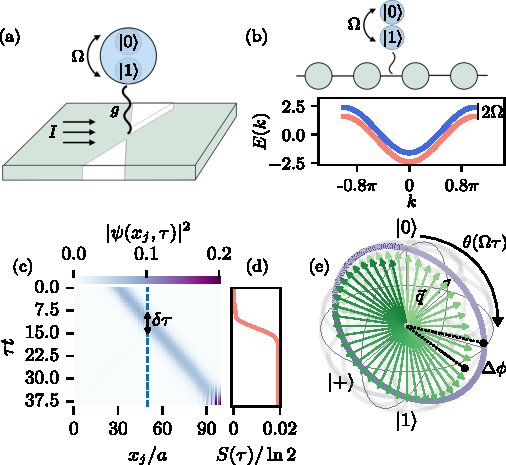
\includegraphics[width=1.0\linewidth]{Figures/fig1.pdf}
    \caption{(a) Sketch of a typical experimental setup for the measurement of a qubit using a QPC. The QPC is a 2 dimensional electron gas separated by a constriction, through which the  current $I$ is flowing due to a voltage bias. The qubit is implemented as a double quantum dot, capacitively coupled to the QPC current. (b) Representation of the Hamiltonian model in Eq. \eqref{eq:qpc_dd_H}, with the eigenenergies of the decoupled qubit $\epsilon_\pm$ and $E(k)$ from Eq.\eqref{eq:decoupled_energies} also depicted.}
    \label{fig:fig1}
\end{figure}

% THIS IS COMMENTED OUT FOR NOW
\iffalse
\begin{figure} \centering \subfloat[]{% 
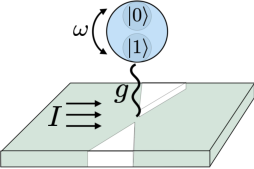
\includegraphics[width=0.5\linewidth]{Figures/exp_model.pdf} \label{fig:exp_model} } \subfloat[]{% 
\includegraphics[width=0.5\linewidth]{Figures/h_model.pdf} \label{fig:h_model} } \\[1em] \subfloat[]{%
\includegraphics[width=0.6\linewidth]{Figures/qpc_trajectories.pdf}% 
\label{fig:qpc_trajectories} } \subfloat[]{% 
\includegraphics[width=0.4\linewidth]{Figures/bloch_orbit_edit.pdf}% 
\label{fig:bloch_sphere} } 
\caption{(a) Diagram of the model in Eq.\eqref{eq:qpc_dd_H}, the QPC particle is represented as a Gaussian wavepacket and the qubit as a 2-level system. (b) Bloch sphere trajectories for the qubit. The free evolution corresponds to the purple dots and the QPC influenced one to the green arrows (c) Time evolution of the wavepacket in the QPC.}\label{fig:backaction_intuit} 
\end{figure}
\fi
 
\section{Results}

\subsection{Measurement Backaction}\label{sect:backaction}

\begin{itemize}
    \item Time-evolving the initial state $\ket{\Psi}$ with ED yields the qubit's reduced density matrix $\hat{\rho}_q(\tau)$ and from it, the post-measurement phase gain $\Delta \phi$ and entanglement entropy $S$. 

    \item Three distinct behaviors are observed in Figs.\ref{fig:fig2}(a) and (b): Slow qubit ($\omega = 0.0001$) with a monotonic decrease in $k_0$, fast qubit ($\omega = 2.0$ ) in which QPC and qubit are decoupled, and intermediate oscillation ($\omega = 0.4$) where both $\Delta \phi$ and $S$ are non-monotonic. We refer to these as quasi-static, Floquet and coherent regimes respectively.

    % \item The difference between Rabi frequencies is explained with a generalization to von Neumann's scheme, where time evolution is divided into three intervals: Before the measurement ($\tau<0$) and after the measurement ($\tau>\delta\tau$) where the time evolution is given solely by $\hat{H}_0$, and during the measurement ($0\leq\tau\leq\delta\tau$) when $\hat{H}_I$ dictates the evolution \cite{siddiqi2024}. (See Apendix \ref{app:derivation_backaction}).
    
    \item The dashed lines were calculated from the qubit's reduced density matrix, obtained via a generalized von Neumann measurement scheme\cite{siddiqi2024}, by assuming small $\tilde{g} = g\delta \tau$ and $\delta \tau \omega \ll \tilde{g}\ll 1 $, in order to simplify the entanglement operator during measurement (See Apendix \ref{app:derivation_backaction}).

    \item The leading order term is the phase gain Eq.\eqref{eq:phase_gain} and the second order term yields the dephasing factor Eq.\eqref{eq:dephasing_factor}, which generates an exponential decrease of the Bloch vector's magnitude, thus explaining the entanglement. 
\end{itemize}


\begin{align}\label{eq:phase_gain}
    \Delta \phi (k_0)= g/(J\sqrt{2\pi}\tan{(ak_0)}) 
\end{align}

\begin{align}\label{eq:dephasing_factor}
    R(k_0) =\exp{ -g^2 J\sin{(2ak_0)}\Delta(k_0)/(\sqrt{2\pi} v_g^2)}
\end{align}
\begin{itemize}
     \item The expression for $\Delta \phi (k_0)$ and $R(k_0)$ are consistent with continuous measurement and the quasi-static regime, but fail to predict the non-monotonic effects, as $\omega$ is increased. 

     \item A broader view of the three backaction regimes in terms of the the entropy is shown in Fig.\ref{fig:fig2}, with boundaries between the slow qubit (I), coherent (II) and Floquet (II) regimes included. This figure indicates that the enhanced measurement peak is only observed in regime (II). 
     
     \item In the following, we explain the mechanism behind the measurement enhancement and derive the expressions for the boundaries between the three regimes from the entanglement entropy and perturbative corrections.
\end{itemize}

\begin{figure*}
  \centering
    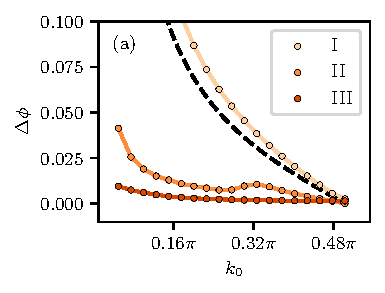
\includegraphics[width=0.6\linewidth]{Figures/phase_v_k0.pdf}
    \includegraphics[width=0.6\linewidth]{Figures/entropy_vs_K0_and_om.png}%
  \caption{Measurement induced backaction and entanglement on the qubit. (a)-(b) Phase gain and entanglement as a function of $k_0$ for three different Rabi frequencies. ED results are shown as red dots and the dashed lines were obtained with Eq.\eqref{eq:phase_gain} and Eq.\eqref{eq:dephasing_factor}. (c) Color map for the entropy as a unction of $k_0$ and $\omega$, the dashed lines  indicate the boundaries between regimes. The points marked with the star symbols correspond to each other in both figures.}\label{fig:fig2}
\end{figure*}


\subsection{Entanglement Entropy}


\begin{figure}
    \centering
    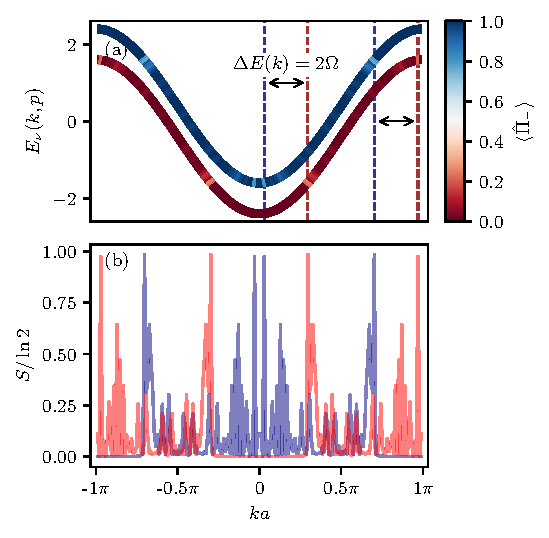
\includegraphics[width=0.8\linewidth]{Figures/band_struct_main.pdf}
    \caption{ED band structure and entanglement for $\omega = 0.4J$ separated into symmetric (Blue), anti-symmetric (red) and labeled by momentum k. (a) Entanglement of each eigenvector of $\hat{H}$. (b) Eigenenergies colored by the projection onto the symmetric band of their respective eigenvectors. The vertical lines indicate the 4 most entangled eigenstates, where dashed/solid lines indicating the resonance.}\label{fig:fig3}
\end{figure}

\begin{itemize}
    \item The processes that dominate each of region are read from the perturbative corrections (See Appendix \ref{app:derivation_perturbative}) in Eq.\eqref{eq:psi_first_order}, where greek indices indicate the band label $\pm$, $\mu \neq \nu$ always, and $\xi(k,p) = \sin{(x_bk)}\sin{(x_b p+p)}\sin{(x_b p)}\sin{(x_b k+k)}$.

    \item We focus on the second term, which gives Eq.\eqref{eq:entropy_bounds} corresponding to the vertical lines in Fig. \ref{fig:fig2}.

    \item Fig.\ref{fig:fig3}, shows that states that fulfill the degeneracy condition in its denominator are the most entangled ones, which explains the resonant line in the coherent regime (II): The gaussian weights of the wave packet select the eigenstates that contribute during measurement.
\end{itemize}

\begin{widetext}
\begin{equation}
    \ket{\Psi_\nu^{(1)} (k)} = \frac{1}{N+1} \sum_{p \neq k} \ket{p} \otimes \left\{\frac{\xi(k,p)}{-2J(\cos k - \cos p)} \ket{\nu} + \frac{\xi(k,p)}{2\epsilon_\nu - 2J(\cos k - \cos p)} \ket{\mu} \right\} + \frac{1}{N+1} \frac{\xi(k,k)}{2\epsilon_\nu} \ket{k} \otimes \ket{\mu}\label{eq:psi_first_order}
\end{equation}
\end{widetext}


\begin{subequations}\label{eq:entropy_bounds}
\begin{align}
    2\omega < \text{min}\Delta E (k)
\end{align}
\begin{align}
    \omega  > J  
\end{align}
\end{subequations}


\section{Discussion and Outlook}

\begin{itemize}
    \item We proposed a simple Hamiltonian model for the
    QPC-qubit measurement process, with main parameters $k_0$, $\omega$, that allows us to go beyond the typical current based calculations, and maintain unitary dynamics.

    \item  We find 3 regimes by looking at the entanglement and backaction: quasi-static, coherent and
    Floquet, and identified the entropy generating processes via the degeneracies of the perturbative corrections.

    \item The coherent regime exhibits unique behavior, characterized by a resonant degeneracy between the QPC's kinetic energy and the band-gap between qubit states, that is not possible in the quasi-static and Floquet regimes.

    \item Furthermore, the individual terms in the corrections can be interpreted as different processes: The first, represents scattering off a constant potential, the second is inelastic scattering that generates an excitation in the qubit \cite{elistratovTheoryWave2023} and the third is the static qubit's residual cotribution.

    \item The inelastic scattering interpretation is supported by our derivation of Eq.\eqref{eq:von_neumann_H}, where we neglected corrections with a factor of $\omega \delta \tau$ that contain bit flip processes.

    \item This two channel scattering is similar to those found in Fano resonances where the interference between a scattering channel within a continuum and a secondary channel that results in an excitation in a discrete state results in a resonant effect, most clearly observed in a peak (or dip) in transmision \cite{kobayashiFano2004}.

    \item In this sense, the resonant line can be traced to the existence of novel many-body effects in QPC's interacting with small systems \cite{ouyangBackaction2010, youngInelasticBackaction2010, snymanPolarization2007}.

    \item We expect that our results should be seen in experiments when the bias (...).

    \item To further elaborate on the many body connection, our model and methodology can be extended to sequences of wavepackets interacting with the qubit one after the other, which also opens up the possibility of implementing tests for Legget-Garg inequalities \cite{jordan2008}.

    \item In addtion, our methodology can be generalized to spin and valley degrees of freedom, relevant to silicon/germanium based quantum dot qubits.
\end{itemize}

\section{Acknowledgments}

This project was funded by (...)

\bibliographystyle{apsrev4-2} % APS recommended BibTeX style
\bibliography{qpc}     % Name of your .bib file (witho

\appendix 

\section{Numerical Setup and Finite Size Effects}\label{app:numerical_setup}

\section{Von Neumann's Measurement Scheme}\label{app:derivation_backaction}

\begin{itemize}
    \item This section starts with explaining VN and relating it with Gurvitz and Korotkov are expected to fit.     
    \item Then derive the toy model.

    \item Applying $\hat{U}$ to $\ket{\Psi}$ results in an entangled state Eq.\eqref{eq:entangled_state} where $\hat{O}$ is correlated with the occupation in the qubit. 
    
    \item Tracing away the QPC degrees of freedom, yields the post measurement qubit density matrix $\hat{\rho}^\prime$ in terms of the Bloch vector in Eq.\eqref{eq:new_q}, with the phase gain $\Delta \phi$ in Eq.\eqref{eq:phase_gain} and dephasing factor $R$ in Eq.\eqref{eq:dephasing_factor}.
\end{itemize}

\begin{subequations}\label{eq:von_neumann_H}
    \begin{align}
    \hat{U} \approx e^{-i \tilde{g}\hat{n}_1 \otimes \hat{c}^\dagger_{b+}\hat{c}_b + h.c.} e^{-i \tilde{g}^2 \hat{n}_1 \otimes \hat{O}},
\end{align}

\begin{align}
    \hat{O} = (\hat{c}^\dagger_{b+2}\hat{c}_{b} +\hat{c}^\dagger_{b-1}\hat{c}_{b+1} - \text{h.c})
\end{align}
\end{subequations}

\begin{align}\label{eq:entangled_state}
    \ket{\Psi (\delta\tau} = & \ket{\psi(\delta \tau)} \otimes \cos{(\theta(\tau_b)/2)}\ket{0} +  \nonumber \\ 
    & e^{-i\tilde{g}\hat{O}}\ket{\psi(\delta \tau)} \otimes \sin{(\theta(\tau_b)/2)} e^{i \phi}\ket{1}
\end{align}

\begin{align}\label{eq:new_q}
 \vec{q}^\prime = 
    \begin{pmatrix}
    R(k_0) \sin(\theta(\tau_b)) \cos(\phi - \Delta \phi(k_0)) \\
    R(k_0) \sin(\theta(\tau_b)) \sin(\phi - \Delta \phi(k_0)) \\
    \cos(\theta(\tau_b))
    \end{pmatrix}
\end{align}

\section{Derivation of the Perturbative Corrections}\label{app:derivation_perturbative}

  
\end{document}

